\chapter{Kernels}
\label{chap:Kernels}

\section{Introduction}
So far in this book, we have been assuming that each object that we wish to classify or cluster or process in anyway can be represented as a fixed-size feature vector, typically of the form $\vec{x}_i \in \mathbb{R}^D$. However, for certain kinds of objects, it is not clear how to best represent them as fixed-sized feature vectors. For example, how do we represent a text document or protein sequence, which can be of variable length? or a molecular structure, which has complex 3d geometry? or an evolutionary tree, which has variable size and shape?

One approach to such problems is to define a generative model for the data, and use the inferred latent representation and/or the parameters of the model as features, and then to plug these features in to standard methods. For example, in Chapter 28 TODO, we discuss deep learning, which is essentially an unsupervised way to learn good feature representations.

Another approach is to assume that we have some way of measuring the similarity between objects, that doesn’t require preprocessing them into feature vector format. For example, when comparing strings, we can compute the edit distance between them. Let $\kappa(\vec{x},\vec{x}') \geq 0$ be some measure of similarity between objects $\kappa(\vec{x},\vec{x}') \in \mathcal{X}$,  we will call $\kappa$ a \textbf{kernel function}. Note that the word “kernel” has several meanings; we will discuss a different interpretation in Section 14.7.1 TODO.

In this chapter, we will discuss several kinds of kernel functions. We then describe some algorithms that can be written purely in terms of kernel function computations. Such methods can be used when we don’t have access to (or choose not to look at) the “inside” of the objects $\vec{x}$ that we are processing.


\section{Kernel functions}
\begin{definition}
A \textbf{kernel function}\footnote{\url{http://en.wikipedia.org/wiki/Kernel_function}} is a real-valued function of two arguments, $\kappa(\vec{x},\vec{x}') \in \mathbb{R}$. Typically the function is symmetric (i.e., $\kappa(\vec{x},\vec{x}')=\kappa(\vec{x}',\vec{x})$, and non-negative (i.e., $\kappa(\vec{x},\vec{x}') \geq 0$). 
\end{definition}

We give several examples below.

\subsection{RBF kernels}
The \textbf{Gaussian kernel} or \textbf{squared exponential kernel}(SE kernel) is defined by
\begin{equation}
\kappa(\vec{x},\vec{x}')=\exp\left(-\frac{1}{2}(\vec{x}-\vec{x}')^T\vec{\Sigma}^{-1}(\vec{x}-\vec{x}')\right)
\end{equation}

If $\vec{\Sigma}$ is diagonal, this can be written as
\begin{equation}
\kappa(\vec{x},\vec{x}')=\exp\left(-\frac{1}{2}\sum\limits_{j=1}^D \frac{1}{\sigma_j^2}(x_j-x_j')^2\right)
\end{equation}

We can interpret the $\sigma_j$ as defining the \textbf{characteristic length scale} of dimension $j$.If $\sigma_j = \infty$, the corresponding dimension is ignored; hence this is known as the \textbf{ARD kernel}. If $\vec{\Sigma}$ is spherical, we get the isotropic kernel
\begin{equation}\label{eqn:RBF-kernel}
\kappa(\vec{x},\vec{x}')=\exp\left(-\frac{\lVert\vec{x}-\vec{x}'\rVert^2}{2\sigma^2}\right)
\end{equation}

Here $\sigma^2$ is known as the \textbf{bandwidth}. Equation \ref{eqn:RBF-kernel} is an example of a \textbf{radial basis function} or \textbf{RBF} kernel, since it is only a function of $\lVert\vec{x}-\vec{x}'\rVert^2$.


\subsection{TF-IDF kernels}
\begin{equation}\label{eqn:RBF-kernel}
\kappa(\vec{x},\vec{x}')=\frac{\phi(\vec{x})^T\phi(\vec{x}')}{\lVert\phi(vec{x})\rVert_2\lVert\phi(\vec{x}')\rVert_2}
\end{equation}
where $\phi(\vec{x})=\text{tf-idf}(\vec{x})$.

\subsection{Mercer (positive definite) kernels}
\label{sec:Mercer-kernels}
If the kernel function satisfies the requirement that the \textbf{Gram matrix}, defined by
\begin{equation}
\vec{K} \triangleq \left(\begin{array}{ccc}
\kappa(\vec{x}_1,\vec{x}_2) & \cdots \kappa(\vec{x}_1,\vec{x}_N) \\
\vdots & \vdots & \vdots \\
\kappa(\vec{x}_N,\vec{x}_1) & \cdots \kappa(\vec{x}_N,\vec{x}_N) 
\end{array}\right)
\end{equation}
be positive definite for any set of inputs $\{\vec{x}_i\}_{i=1}^N$. We call such a kernel a \textbf{Mercer kernel},or \textbf{positive definite kernel}.

If the Gram matrix is positive definite, we can compute an eigenvector decomposition of it as follows
\begin{equation}
\vec{K}=\vec{U}^T\vec{\Lambda}\vec{U}
\end{equation}

where $\vec{\Lambda}$ is a diagonal matrix of eigenvalues $\lambda_i >0$. Now consider an element of $\vec{K}$:
\begin{equation}
k_{ij}=(\vec{\Lambda}^{\frac{1}{2}}\vec{U}_{:,i})^T(\vec{\Lambda}^{\frac{1}{2}}\vec{U}_{:,j})
\end{equation}

Let us define $\phi(\vec{x}_i)=\vec{\Lambda}^{\frac{1}{2}}\vec{U}_{:,i}$, then we can write
\begin{equation}
k_{ij}=\phi(\vec{x}_i)^T\phi(\vec{x}_j)
\end{equation}

Thus we see that the entries in the kernel matrix can be computed by performing an inner product of some feature vectors that are implicitly defined by the eigenvectors $\vec{U}$. In general, if the kernel is Mercer, then there exists a function $\phi$ mapping $\vec{x} \in \mathcal{X}$ to $\mathbb{R}^D$ such that
\begin{equation}
\kappa(\vec{x},\vec{x}')=\phi(\vec{x})^T\phi(\vec{x}')
\end{equation}
where $\phi$ depends on the eigen functions of $\kappa$(so $D$ is a potentially infinite dimensional space).

For example, consider the (non-stationary) \textbf{polynomial kernel} $\kappa(\vec{x},\vec{x}')=(\gamma \vec{x}\vec{x}'+r)^M$, where $r>0$. One can show that the corresponding feature vector $\phi(\vec{x})$ will contain all terms up to degree $M$. For example, if $M=2, \gamma=r=1$ and $\vec{x}, \vec{x}' \in \mathbb{R}^2$, we have
\begin{align*}
(\vec{x}\vec{x}'+1)^2 & =(1+x_1x_1'+x_2+x_2')^2 \\
    & = 1+2x_1x_1'+2x_2x_2'+(x_1x_1')^2+(x_2x_2')^2x_1x_1'x_2x_2' \\
	& = \phi(\vec{x})^T\phi(\vec{x}') \\
\text{where } & \phi(\vec{x})=(1,\sqrt{2}x_1,\sqrt{2}x_2,x_1^2,x_2^2,\sqrt{2}x_1x_2)
\end{align*}

In the case of a Gaussian kernel, the feature map lives in an infinite dimensional space. In such a case, it is clearly infeasible to explicitly represent the feature vectors.

In general, establishing that a kernel is a Mercer kernel is difficult, and requires techniques from functional analysis. However, one can show that it is possible to build up new Mercer kernels from simpler ones using a set of standard rules. For example, if $\kappa_1$ and $\kappa_2$ are both Mercer, so is $\kappa(\vec{x},\vec{x}')=\kappa_1(\vec{x},\vec{x}')+\kappa_2(\vec{x},\vec{x}')=$. See e.g., (Schoelkopf and Smola 2002) for details.


\subsection{Linear kernels}
\begin{equation}
\kappa(\vec{x},\vec{x}')=\vec{x}^T\vec{x}'
\end{equation}

\subsection{Matern kernels}
The \textbf{Matern kernel}, which is commonly used in Gaussian process regression (see Section 15.2), has the following form
\begin{equation}
\kappa(r)=\frac{2^{1-\nu}}{\Gamma(\nu)}\left(\frac{\sqrt{2\nu}r}{\ell}\right)^{\nu}K_{\nu}\frac{\sqrt{2\nu}r}{\ell}
\end{equation}
where $r=\lVert\vec{x}-\vec{x}'\rVert$, $\nu>0$, $\ell>0$, and $K_{\nu}$ is a modified Bessel function. As $\nu \rightarrow \infty$, this approaches the SE kernel. If $\nu=\frac{1}{2}$, the kernel simplifies to
\begin{equation}
\kappa(r)=\exp(-r/\ell)
\end{equation}

If $D=1$, and we use this kernel to define a Gaussian process (see Chapter 15 TODO), we get the \textbf{Ornstein-Uhlenbeck process}, which describes the velocity of a particle undergoing Brownian motion (the corresponding function is continuous but not differentiable, and hence is very “jagged”).


\subsection{String kernels}
\label{sec:String-kernels}
Now let $\phi_s(\vec{x})$ denote the number of times that substrings appears in string $\vec{x}$. We define the kernel between two strings $\vec{x}$ and $\vec{x}'$ as
\begin{equation}
\kappa(\vec{x},\vec{x}')=\sum\limits_{s \in \mathcal{A}^*} w_s\phi_s(\vec{x})\phi_s(\vec{x}')
\end{equation}
where $w_s \geq 0$ and $\mathcal{A}^*$ is the set of all strings (of any length) from the alphabet $\mathcal{A}$(this is known as the Kleene star operator). This is a Mercer kernel, and be computed in $O(|\vec{x}|+|\vec{x}'|)$ time (for certain settings of the weights $\{ws\}$) using suffix trees (Leslie et al. 2003; Vishwanathan and Smola 2003; Shawe-Taylor and Cristianini 2004).

There are various cases of interest. If we set $w_s =0$for $|s| >1$ we get a bag-of-characters kernel. This defines $\phi(\vec{x})$ to be the number of times each character in $\mathcal{A}$ occurs in $\vec{x}$.If we require $s$ to be bordered by white-space, we get a bag-of-words kernel, where $\phi(\vec{x})$ counts how many times each possible word occurs. Note that this is a very sparse vector, since most words will not be present. If we only consider strings of a fixed lengthk, we get the \textbf{k-spectrum} kernel. This has been used to classify proteins into SCOP superfamilies (Leslie et al. 2003).


\subsection{Pyramid match kernels}
% \begin{figure}[hbtp]
% \centering
%     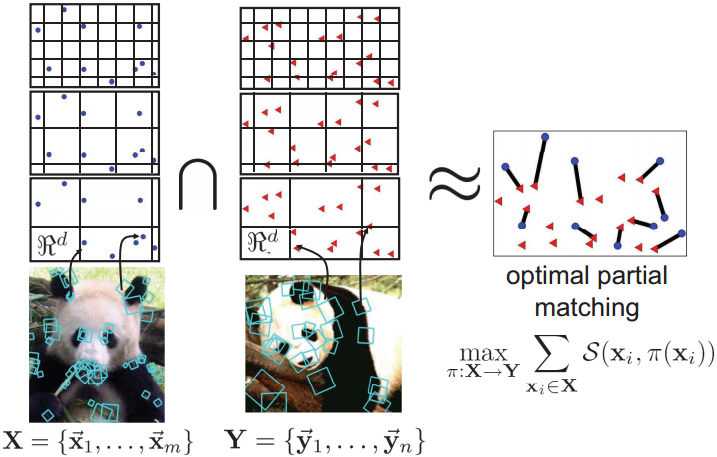
\includegraphics[scale=.70]{pyramid-match-kernel.png}
% \caption{Illustration of a pyramid match kernel computed from two images. Used with kind permission of Kristen Grauman.}
% \label{fig:pyramid-match-kernel}
% \end{figure}


\subsection{Kernels derived from probabilistic generative models}
Suppose we have a probabilistic generative model of feature vectors, $p(\vec{x}|\vec{\theta})$. Then there are several ways we can use this model to define kernel functions, and thereby make the model suitable for discriminative tasks. We sketch two approaches below.


\subsubsection{Probability product kernels}
\begin{equation}\label{eqn:Probability-product-kernels}
\kappa(\vec{x}_i,\vec{x}_j)=\int p(\vec{x}|\vec{x}_i)^{\rho}p(\vec{x}|\vec{x}_j)^{\rho}\mathrm{d}\vec{x}
\end{equation}
where $\rho>0$, and $p(\vec{x}|\vec{x}_i)$ is often approximated by $p(\vec{x}|\hat{\vec{\theta}}(\vec{x}_i))$,where $\hat{\vec{\theta}}(\vec{x}_i)$ is a parameter estimate computed using a single data vector. This is called a \textbf{probability product kernel}(Jebara et al. 2004).

Although it seems strange to fit a model to a single data point, it is important to bear in mind that the fitted model is only being used to see how similar two objects are. In particular, if we fit the model to $\vec{x}_i$ and then the model thinks $\vec{x}_j$ is likely, this means that $\vec{x}_i$ and $\vec{x}_j$ are similar. For example, suppose $p(\vec{x}|\vec{\theta}) \sim \mathcal{N}(\vec{\mu},\sigma^2\vec{I})$, where $\sigma^2$ is fixed. If $\rho=1$, and we use $\hat{\vec{\mu}}(\vec{x}_i)=\vec{x}_i$ and $\hat{\vec{\mu}}(\vec{x}_j)=\vec{x}_j$, we find (Jebara et al. 2004, p825) that
\begin{equation}
\kappa(\vec{x}_i,\vec{x}_j)=\frac{1}{(4\pi\sigma^2)^{D/2}}\exp\left(-\frac{1}{4\sigma^2}\lVert\vec{x}_i-\vec{x}_j\rVert^2\right)
\end{equation}
which is (up to a constant factor) the RBF kernel.

It turns out that one can compute Equation \ref{eqn:Probability-product-kernels} for a variety of generative models, including ones with latent variables, such as HMMs. This provides one way to define kernels on variable length sequences. Furthermore, this technique works even if the sequences are of real-valued vectors, unlike the string kernel in Section \ref{sec:String-kernels}. See (Jebara et al. 2004) for further details


\subsubsection{Fisher kernels}
A more efficient way to use generative models to define kernels is to use a \textbf{Fisher kernel} (Jaakkola and Haussler 1998) which is defined as follows:
\begin{equation}
\kappa(\vec{x}_i,\vec{x}_j)=g(\vec{x}_i)^T\vec{F}^{-1}g(\vec{x}_j)
\end{equation}
where $g$ is the gradient of the log likelihood, or \textbf{score vector}, evaluated at the MLE $\hat{\vec{\theta}}$
\begin{equation}
g(\vec{x}) \triangleq \frac{\mathrm{d}}{\mathrm{d}\vec{\theta}}\log p(\vec{x}|\vec{\theta})|_{\hat{\vec{\theta}}}
\end{equation}
and $\vec{F}$ is the Fisher information matrix, which is essentially the Hessian:
\begin{equation}
\vec{F} \triangleq \left[\frac{\partial^2}{\partial \theta_i \partial \theta_j}\log p(\vec{x}|\vec{\theta})\right]|_{\hat{\vec{\theta}}}
\end{equation}

Note that $\hat{\vec{\theta}}$ is a function of all the data, so the similarity of $\vec{x}_i$ and $\vec{x}_j$ is computed in the context of all the data as well. Also, note that we only have to fit one model.


\section{Using kernels inside GLMs}


\subsection{Kernel machines}
We define a \textbf{kernel machine} to be a GLM where the input feature vector has the form
\begin{equation}\label{eqn:kernel-machine}
\phi(\vec{x})=(\kappa(\vec{x},\vec{\mu}_1),\cdots,\kappa(\vec{x},\vec{\mu}_K))
\end{equation}

where $\vec{\mu}_k \in \mathcal{X}$ are a set of $K$ centroids. If $\kappa$ is an RBF kernel, this is called an \textbf{RBF network}. We discuss ways to choose the $\vec{\mu}_k$ parameters below. We will call Equation \ref{eqn:kernel-machine} a \textbf{kernelised feature vector}. Note that in this approach, the kernel need not be a Mercer kernel.

We can use the kernelized feature vector for logistic regression by defining $p(y|\vec{x},\vec{\theta})=\mathrm{Ber}(y|\vec{w}^T\phi(\vec{x}))$. This provides a simple way to define a non-linear decision boundary. For example, see Figure \ref{fig:kenel-machine-xor}.

\begin{figure}[hbtp]
\centering
\subfloat[]{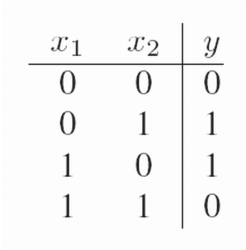
\includegraphics[scale=.70]{kenel-machine-xor-a.png}} \\
\subfloat[]{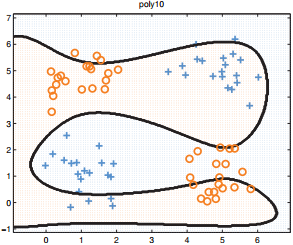
\includegraphics[scale=.70]{kenel-machine-xor-b.png}} \\
\subfloat[]{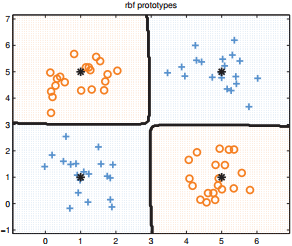
\includegraphics[scale=.70]{kenel-machine-xor-c.png}}
\caption{(a) xor truth table. (b) Fitting a linear logistic regression classifier using degree 10 polynomial expansion. (c) Same model, but using an RBF kernel with centroids specified by the 4 black crosses.}
\label{fig:kenel-machine-xor} 
\end{figure}

We can also use the kernelized feature vector inside a linear regression model by defining $p(y|\vec{x},\vec{\theta})=\mathcal{N}(y|\vec{w}^T\phi(\vec{x}),\sigma^2)$. 


\subsection{L1VMs, RVMs, and other sparse vector machines}
\label{sec:sparse-kernel-machines}
The main issue with kernel machines is: how do we choose the centroids $\vec{\mu}_k$? We can use \textbf{sparse vector machine}, \textbf{L1VM}, \textbf{L2VM}, \textbf{RVM}, \textbf{SVM}.

% In Figure \ref{fig:L2VM-L1VM-RVM-SVM-2d}, we compare L2VM, L1VM, RVM and an SVM using the same RBF kernel on a binary classification problem in 2d.

% \begin{figure}[hbtp]
% \centering
% \subfloat[]{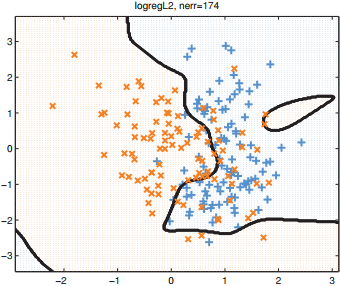
\includegraphics[scale=.50]{L2VM-L1VM-RVM-SVM-2d-a.png}} \\
% \subfloat[]{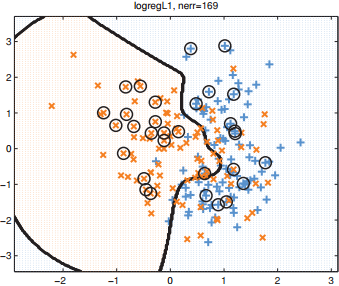
\includegraphics[scale=.50]{L2VM-L1VM-RVM-SVM-2d-b.png}} \\
% \subfloat[]{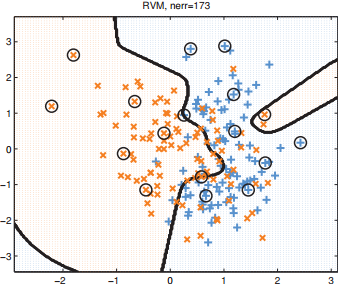
\includegraphics[scale=.50]{L2VM-L1VM-RVM-SVM-2d-c.png}} \\
% \subfloat[]{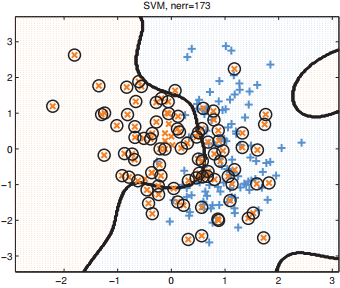
\includegraphics[scale=.50]{L2VM-L1VM-RVM-SVM-2d-d.png}}
% \caption{Example of non-linear binary classification using an RBF kernel with bandwidth $\sigma=0.3$. (a) L2VM with $\lambda=5$. (b) L1VM with $\lambda=1$. (c) RVM. (d) SVM with $C=1/\lambda$ chosen by cross validation. Black circles denote the support vectors.}
% \label{fig:L2VM-L1VM-RVM-SVM-2d} 
% \end{figure}

% In Figure \ref{fig:L2VM-L1VM-RVM-SVM-1d}, we compare L2VM, L1VM, RVM and an SVM using an RBF kernel on a 1d regression problem. 
% \begin{figure}[hbtp]
% \centering
%     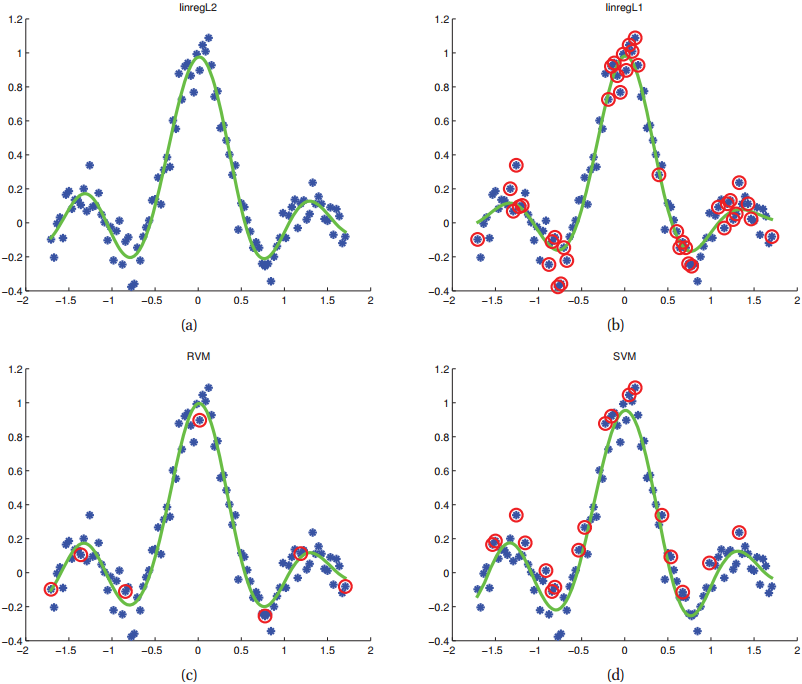
\includegraphics[scale=.70]{L2VM-L1VM-RVM-SVM-1d.png}
% \caption{Example of kernel based regression on the noisy sinc function using an RBF kernel with bandwidth $\sigma=0.3$. (a) L2VM with $\lambda=0.5$. (b) L1VM with $\lambda=0.5$. (c) RVM. (d) SVM regression with $C=1/\lambda$ chosen by cross validation, and $\epsilon=0.1$ (the default for SVMlight). Red circles denote the retained training exemplars.}
% \label{fig:L2VM-L1VM-RVM-SVM-1d} 
% \end{figure}


\section{The kernel trick}
Rather than defining our feature vector in terms of kernels, $\phi(\vec{x})=(\kappa(\vec{x},\vec{x}_1),\cdots,\kappa(\vec{x},\vec{x}_N))$, we can instead work with the original feature vectors $\vec{x}$, but modify the algorithm so that it replaces all inner products of the form $<\vec{x}_i,\vec{x}_j>$ with a call to the kernel function, $\kappa(\vec{x}_i,\vec{x}_j)$. This is called the \textbf{kernel trick}. It turns out that many algorithms can be kernelized in this way. We give some examples below. Note that we require that the kernel be a Mercer kernel for this trick to work.


\subsection{Kernelized KNN}
The Euclidean distance can be unrolled as
\begin{equation}\label{eqn:Euclidean-distance}
\lVert\vec{x}_i-\vec{x}_j\rVert=<\vec{x}_i,\vec{x}_i>+<\vec{x}_j,\vec{x}_j>-2<\vec{x}_i,\vec{x}_j>
\end{equation}
then by replacing all $<\vec{x}_i,\vec{x}_j>$ with $\kappa(\vec{x}_i,\vec{x}_j)$ we get Kernelized KNN.


\subsection{Kernelized K-medoids clustering}
\textbf{K-medoids algorothm} is similar to K-means(see Section \ref{sec:K-means}), but instead of representing each cluster’s centroid by the mean of all data vectors assigned to this cluster, we make each centroid be one of the data vectors themselves. Thus we always deal with integer indexes, rather than data objects.

This algorithm can be kernelized by using Equation \ref{eqn:Euclidean-distance} to replace the distance computation.


\subsection{Kernelized ridge regression}
Applying the kernel trick to distance-based methods was straightforward. It is not so obvious how to apply it to parametric models such as ridge regression. However, it can be done, as we now explain. This will serve as a good “warm up” for studying SVMs.


\subsubsection{The primal problem}
we rewrite Equation \ref{eqn:Ridge-regression-J} as the following
\begin{equation}\label{eqn:Ridge-regression-primal-form}
J(\vec{w})=(\vec{y}-\vec{X}\vec{w})^T(\vec{y}-\vec{X}\vec{w})+\lambda\lVert\vec{w}\rVert^2
\end{equation}
and its solution is given by Equation \ref{eqn:Ridge-regression-solution}.


\subsubsection{The dual problem}
Equation \ref{eqn:Ridge-regression-primal-form} is not yet in the form of inner products. However, using the matrix inversion lemma (Equation 4.107 TODO) we rewrite the ridge estimate as follows
\begin{equation}
\vec{w}=\vec{X}^T(\vec{X}\vec{X}^T+\lambda\vec{I}_N)^{-1}\vec{y}
\end{equation}
which takes $O(N^3+N^2D)$ time to compute. This can be advantageous if $D$ is large. Furthermore, we see that we can partially kernelize this, by replacing $\vec{X}\vec{X}^T$ with the Gram matrix $\vec{K}$. But what about the leading $\vec{X}^T$ term?

Let us define the following \textbf{dual variables}:
\begin{equation}
\vec{\alpha}=(\vec{K}+\lambda\vec{I}_N)^{-1}\vec{y}
\end{equation}

Then we can rewrite the \textbf{primal variables} as follows
\begin{equation}
\vec{w}=\vec{X}^T\vec{\alpha}=\sum\limits_{i=1}^N \alpha_i\vec{x}_i
\end{equation}

This tells us that the solution vector is just a linear sum of the $N$ training vectors. When we plug this in at test time to compute the predictive mean, we get
\begin{equation}
y=f(\vec{x})=\sum\limits_{i=1}^N \alpha_i\vec{x}_i^T\vec{x}=\sum\limits_{i=1}^N \alpha_i\kappa(\vec{x}_i,\vec{x})
\end{equation}

So we have succesfully kernelized ridge regression by changing from primal to dual variables. This technique can be applied to many other linear models, such as logistic regression.


\subsubsection{Computational cost}
The cost of computing the dual variables $\vec{\alpha}$ is $O(N^3)$, whereas the cost of computing the primal variables $\vec{w}$ is $O(D^3)$. Hence the kernel method can be useful in high dimensional settings, even if we only use a linear kernel (c.f., the SVD trick in Equation \ref{eqn:Ridge-regression-SVD}). However, prediction using the dual variables takes $O(ND)$ time, while prediction using the primal variables only takes $O(D)$ time. We can speedup prediction by making $\vec{\alpha}$ sparse, as we discuss in Section \ref{sec:SVMs}.


\subsection{Kernel PCA}
TODO


\section{Support vector machines (SVMs)}
\label{sec:SVMs}
In Section \ref{sec:sparse-kernel-machines}, we saw one way to derive a sparse kernel machine, namely by using a GLM with kernel basis functions, plus a sparsity-promoting prior such as $\ell_1$ or ARD. An alternative approach is to change the objective function from negative log likelihood to some other loss function, as we discussed in Section \ref{sec:Surrogate-loss-functions}. In particular, consider the $\ell_2$ regularized empirical risk function
\begin{equation}
J(\vec{w}, \lambda)=\sum\limits{i=1}^N L(y_i, \hat{y_i})+\lambda\lVert\vec{w}\rVert^2
\end{equation}
where $\hat{y_i}=\vec{w}^T\vec{x}_i+w_0$.

If $L$ is quadratic loss, this is equivalent to ridge regression, and if $L$ is the log-loss defined in Equation \ref{eqn:log-loss}, this is equivalent to logistic regression.

However, if we replace the loss function with some other loss function, to be explained below, we can ensure that the solution is sparse, so that predictions only depend on a subset of the training data, known as \textbf{support vectors}. This combination of the kernel trick plus a modified loss function is known as a \textbf{support vector machine} or \textbf{SVM}. 

Note that SVMs are very unnatural from a probabilistic point of view. 
\begin{itemize}
\item{First, they encode sparsity in the loss function rather than the prior.}
\item{Second, they encode kernels by using an algorithmic trick, rather than being an explicit part of the model. }
\item{Finally, SVMs do not result in probabilistic outputs, which causes various difficulties, especially in the multi-class classification setting (see Section 14.5.2.4 TODO for details).}
\end{itemize}

It is possible to obtain sparse, probabilistic, multi-class kernel-based classifiers, which work as well or better than SVMs, using techniques such as the L1VM or RVM, discussed in Section \ref{sec:sparse-kernel-machines}. However, we include a discussion of SVMs, despite their non-probabilistic nature, for two main reasons. 
\begin{itemize}
\item{First, they are very popular and widely used, so all students of machine learning should know about them.}
\item{Second, they have some computational advantages over probabilistic methods in the structured output case; see Section 19.7 TODO.}
\end{itemize}


\subsection{SVMs for classification}


\subsubsection{Primal form}
\textbf{Representation}
\begin{equation}
\mathcal{H}:y=f(\vec{x})=\text{sign}(\vec{w}\vec{x}+b)
\end{equation}

\textbf{Evaluation}
\begin{eqnarray}
\min_{\vec{w},b}  && \frac{1}{2}\|\vec{w}\|^2 \\
       & s.t. \quad & y_i(\vec{w}\vec{x}_i+b)\geqslant 1, i=1,2, \dots , N
\end{eqnarray}


\subsubsection{Dual form}
\textbf{Representation}
\begin{equation}
\mathcal{H}:y=f(\vec{x})=\text{sign}\left(\sum\limits_{i=1}^N{\alpha_iy_i(\vec{x} \cdot \vec{x}_i)}+b\right)
\end{equation}

\textbf{Evaluation}
\begin{eqnarray}
 \min_{\alpha} && \frac{1}{2} \sum\limits_{i=1}^N\sum\limits_{j=1}^N \alpha_i\alpha_j y_i y_j (\vec{x}_i \cdot \vec{x}_j) - \sum\limits_{i=1}^N \alpha_i \\
               & s.t.  \quad &\sum\limits_{i=1}^N\alpha_i y_i=0 \\
               && \alpha_i \geqslant 0, i=1,2, \dots, N
\end{eqnarray}


\subsubsection{Primal form with slack variables}
\textbf{Representation}
\begin{equation}
\mathcal{H}:y=f(\vec{x})=\text{sign}(\vec{w}\vec{x}+b)
\end{equation}

\textbf{Evaluation}
\begin{eqnarray}
\min_{\vec{w},b}  &&  C \sum\limits_{i=1}^N\xi_i + \frac{1}{2}\|\vec{w}\|^2 \label{eqn:pfwr1} \\
      & s.t. \quad & y_i(\vec{w}\vec{x}_i+b)\geqslant 1-\xi_i  \label{eqn:pfwr2} \\
                  && \xi_i \geqslant 0, \quad i=1,2, \dots, N \label{eqn:pfwr3}
\end{eqnarray}


\subsubsection{Dual form with slack variables}
\textbf{Representation}
\begin{equation}
\mathcal{H}:y=f(\vec{x})=\text{sign}\left(\sum\limits_{i=1}^N{\alpha_iy_i(\vec{x} \cdot \vec{x}_i)}+b\right)
\end{equation}

\textbf{Evaluation}
\begin{eqnarray}
 \min_{\alpha} && \frac{1}{2} \sum\limits_{i=1}^N\sum\limits_{j=1}^N \alpha_i\alpha_j y_i y_j (\vec{x}_i \cdot \vec{x}_j) - \sum\limits_{i=1}^N \alpha_i \\
               & s.t.  \quad & \sum\limits_{i=1}^N\alpha_i y_i=0 \\
               && 0 \leqslant  \alpha_i \leqslant C, i=1,2, \dots, N
\end{eqnarray}

\begin{eqnarray}
\alpha_i=0 \Rightarrow y_i(\vec{w} \cdot \vec{x}_i+b)\geqslant 1 \\
\alpha_i=C \Rightarrow y_i(\vec{w} \cdot \vec{x}_i+b)\leqslant 1 \\
0<\alpha_i<C \Rightarrow y_i(\vec{w} \cdot \vec{x}_i+b)= 1
\end{eqnarray}


\subsubsection{Hinge Loss}
Linear support vector machines can also be interpreted as hinge loss minimization:
\begin{equation}\label{eqn:Hinge-Loss-objective}
\min_{\vec{w},b} \sum\limits_{i=1}^N{L(y_i,f(\vec{x}_i))} + \lambda\|\vec{w}\|^2
\end{equation}
where $L(y, f(\vec{x}))$ is a \textbf{hinge loss function}:
\begin{equation}
L(y, f(\vec{x})) = \begin{cases}
1-yf(x),  & 1-yf(x) > 0 \\
0,  & 1-yf(x) \leqslant 0
\end{cases}
\end{equation}

\begin{proof}
We can write equation \ref{eqn:Hinge-Loss-objective} as equations \ref{eqn:pfwr1} $\sim$ \ref{eqn:pfwr3}.

Define slack variables
\begin{equation}
\xi_i \triangleq 1-y_i(\vec{w} \cdot \vec{x}_i + b),\xi_i \geqslant 0
\end{equation}

Then $\vec{w},b,\xi_i$ satisfy the constraints \ref{eqn:pfwr1} and \ref{eqn:pfwr2}. And objective function \ref{eqn:pfwr3} can be written as
\begin{equation}
\min_{\vec{w},b} \sum\limits_{i=1}^N{\xi_i}+ \lambda\|\vec{w}\|^2 \nonumber
\end{equation}

If $\lambda=\dfrac{1}{2C}$, then 
\begin{equation}
\min_{\vec{w},b} \dfrac{1}{C}\left(C\sum\limits_{i=1}^N{\xi_i}+\dfrac{1}{2}\|\vec{w}\|^2\right)
\end{equation}
It is equivalent to equation \ref{eqn:pfwr1}.

\end{proof}


\subsubsection{Optimization}
QP, SMO


\subsection{SVMs for regression}


\subsubsection{Representation}
\begin{equation}
\mathcal{H}: y=f(\vec{x})=\vec{w}^T\vec{x}+b
\end{equation}


\subsubsection{Evaluation}
\begin{equation}
J(\vec{w})=C\sum\limits_{i=1}^N L(y_i,f(\vec{x}_i))++\dfrac{1}{2}\lVert\vec{w}\rVert^2
\end{equation}
where $L(y,f(\vec{x}))$ is a \textbf{epsilon insensitive loss function}:
\begin{equation}
L(y,f(\vec{x})) = \begin{cases}
0  & , |y-f(\vec{x})|<\epsilon \\
|y-f(\vec{x})|-\epsilon  & , \text{ otherwise}
\end{cases}
\end{equation}
and $C=1/\lambda$ is a regularization constant. 

This objective is convex and unconstrained, but not differentiable, because of the absolute value function in the loss term. As in Section 13.4 TODO, where we discussed the lasso problem, there are several possible algorithms we could use. One popular approach is to formulate the problem as a constrained optimization problem. In particular, we introduce \textbf{slack variables} to represent the degree to which each point lies outside the tube:
\begin{align*}
y_i \leq & f(\vec{x}_i)+\epsilon+\xi_i^+ \\
y_i \geq & f(\vec{x}_i)-\epsilon-\xi_i^- 
\end{align*}

Given this, we can rewrite the objective as follows:
\begin{equation}
J(\vec{w})=C\sum\limits_{i=1}^N (\xi_i^+ + \xi_i^-)++\dfrac{1}{2}\lVert\vec{w}\rVert^2
\end{equation}
This is a standard quadratic problem in $2N+D+1$ variables.


\subsection{Choosing $C$}
\label{sec:SVM-Choosing-C}
SVMs for both classification and regression require that you specify the kernel function and the parameter $C$. Typically $C$ is chosen by cross-validation. Note, however, that $C$ interacts quite strongly with the kernel parameters. For example, suppose we are using an RBF kernel with precision $\gamma=\frac{1}{2\sigma^2}$. If $\gamma=5$, corresponding to narrow kernels, we need heavy regularization, and hence small $C$(so $\lambda=1/C$is big). If $\gamma=1$, a larger value of $C$should be used. So we see that $\gamma$ and $C$ are tightly coupled. This is illustrated in Figure \ref{fig:choosing-C}, which shows the CV estimate of the 0-1 risk as a function of $C$ and $\gamma$.

\begin{figure}[hbtp]
\centering
\subfloat[]{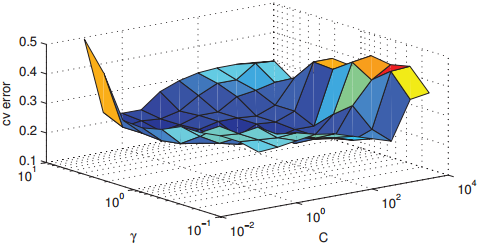
\includegraphics[scale=.50]{choosing-C-a.png}} \\
\subfloat[]{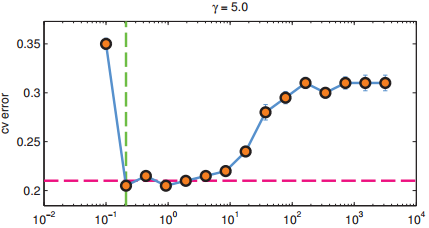
\includegraphics[scale=.50]{choosing-C-b.png}}
\caption{(a) A cross validation estimate of the 0-1 error for an SVM classifier with RBF kernel with different precisions $\gamma=1/(2\sigma^2)$ and different regularizer $\gamma=1/C$, applied to a synthetic data set drawn from a mixture of 2 Gaussians. (b) A slice through this surface for $\gamma=5$ The red dotted line is the Bayes optimal error, computed using Bayes rule applied to the model used to generate the data. Based on Figure 12.6 of (Hastie et al. 2009). }
\label{fig:choosing-C} 
\end{figure}

The authors of libsvm recommend (Hsu et al. 2009) using CV over a 2d grid with values $C \in \{2^{−5},2^{−3},\cdots,2^{15}\}$ and $\gamma \in \{2^{−15},2^{−13},\cdots,2^3\}$. In addition, it is important to standardize the data first, for a spherical Gaussian kernel to make sense.

To choose $C$ efficiently, one can develop a path following algorithm in the spirit of lars (Section 13.3.4 TODO). The basic idea is to start with $\lambda$ large, so that the margin $1/\lVert\vec{w}(\lambda)\rVert$ is wide, and hence all points are inside of it and have $\alpha_i =1$. By slowly decreasing $\lambda$, a small set of points will move from inside the margin to outside, and their $\alpha_i$ values will change from 1 to 0, as they cease to be support vectors. When $\lambda$ is maximal, the function is completely smoothed, and no support vectors remain. See (Hastie et al. 2004) for the details.


\subsection{A probabilistic interpretation of SVMs}
TODO see MLAPP Section 14.5.5


\subsection{Summary of key points}
Summarizing the above discussion, we recognize that SVM classifiers involve three key ingredients: the kernel trick, sparsity, and the large margin principle. The kernel trick is necessary to prevent underfitting, i.e., to ensure that the feature vector is sufficiently rich that a linear classifier can separate the data. (Recall from Section \ref{sec:Mercer-kernels} that any Mercer kernel can be viewed as implicitly defining a potentially high dimensional feature vector.) If the original features are already high dimensional (as in many gene expression and text classification problems), it suffices to use a linear kernel, $\kappa(\vec{x},\vec{x}')=\vec{x}^T\vec{x}'$ , which is equivalent to working with the original features.

The sparsity and large margin principles are necessary to prevent overfitting, i.e., to ensure that we do not use all the basis functions. These two ideas are closely related to each other, and both arise (in this case) from the use of the hinge loss function. However, there are other methods of achieving sparsity (such as $\ell_1$), and also other methods of maximizing the margin(such as boosting). A deeper discussion of this point takes us outside of the scope of this book. See e.g., (Hastie et al. 2009) for more information.


\section{Comparison of discriminative kernel methods}
We have mentioned several different methods for classification and regression based on kernels, which we summarize in Table \ref{tab:Comparison-of-kernel-based-classifiers}. (GP stands for “Gaussian process”, which we discuss in Chapter 15 TODO.) The columns have the following meaning:
\begin{itemize}
\item{Optimize $\vec{w}$: a key question is whether the objective $J(\vec{w}=-\log p(\mathcal{D}|\vec{w})-\log p(\vec{w}))$ is convex or not. L2VM, L1VM and SVMs have convex objectives. RVMs do not. GPs are Bayesian methods that do not perform parameter estimation.}
\item{Optimize kernel: all the methods require that one “tune” the kernel parameters, such as the bandwidth of the RBF kernel, as well as the level of regularization. For methods based on Gaussians, including L2VM, RVMs and GPs, we can use efficient gradient based optimizers to maximize the marginal likelihood. For SVMs, and L1VM, we must use cross validation, which is slower (see Section \ref{sec:SVM-Choosing-C}).}
\item{Sparse: L1VM, RVMs and SVMs are sparse kernel methods, in that they only use a subset of the training examples. GPs and L2VM are not sparse: they use all the training examples. The principle advantage of sparsity is that prediction at test time is usually faster. In addition, one can sometimes get improved accuracy.}
\item{Probabilistic: All the methods except for SVMs produce probabilistic output of the form $p(y|\vec{x})$. SVMs produce a “confidence” value that can be converted to a probability, but such probabilities are usually very poorly calibrated (see Section 14.5.2.3 TODO).}
\item{Multiclass: All the methods except for SVMs naturally work in the multiclass setting, by using a multinoulli output instead of Bernoulli. The SVM can be made into a multiclass classifier, but there are various difficulties with this approach, as discussed in Section 14.5.2.4 TODO.}
\item{Mercer kernel: SVMs and GPs require that the kernel is positive definite; the other techniques do not.}
\end{itemize}

\begin{table}
\centering
\begin{tabular}{llllllll}
\hline\noalign{\smallskip}
Method & Opt. \vec{w} & Opt. & Sparse & Prob. & Multiclass & Non-Mercer & Section \\
\noalign{\smallskip}\svhline\noalign{\smallskip}
L2VM & Convex & EB & No & Yes & Yes & Yes & 14.3.2 \\
L1VM & Convex & CV & Yes & Yes & Yes & Yes & 14.3.2 \\
RVM & Not convex & EB & Yes & Yes & Yes & Yes & 14.3.2 \\
SVM & Convex & CV & Yes & No & Indirectly & No & 14.5 \\
GP & N/A & EB & No & Yes & Yes & No & 15 \\
\noalign{\smallskip}\hline
\end{tabular}
\caption{Comparison of various kernel based classifiers. EB = empirical Bayes, CV = cross validation. See text for details}\label{tab:Comparison-of-kernel-based-classifiers}
\end{table}


\section{Kernels for building generative models}
TODO
